\documentclass[8pt,a4paper,compress]{beamer}

\usepackage{/home/siyer/lib/slides}

\title{Hash Tables}
\date{}

\begin{document}
\begin{frame}
\vfill
\titlepage
\end{frame}

\begin{frame}
\frametitle{Outline}
\tableofcontents
\end{frame}

\section{Hashing}
\begin{frame}[fragile]
\begin{itemize}
\item the basic idea is to save items in a key-indexed array, where the index is a function of the key

\item hash function provides a method for computing an array index from a key

\item issues
\begin{itemize}
\item computing the hash function

\item equality test: method for checking whether two keys are equal

\item collision resolution: algorithm and data structure to handle two keys that hash to the same array index
\end{itemize}

\item classic space-time tradeoff
\begin{itemize}
\item no space limitation: trivial hash function with key as index

\item no time limitation: trivial collision resolution with sequential search

\item space and time limitations: hashing (the real world)
\end{itemize}
\end{itemize}
\end{frame}

\begin{frame}[fragile]
\begin{itemize}
\item idealistic goal: scramble the keys uniformly to produce a table index that is
\begin{itemize}
\item efficiently computable

\item equally likely for each key
\end{itemize}

\item example 1: phone numbers
\begin{itemize}
\item bad: first three digits

\item better: last three digits
\end{itemize}

\item example 2: social security numbers
\begin{itemize}
\item bad: first three digits

\item better: last three digits
\end{itemize}

\item practical challenge: need different approach for each type of key
\end{itemize}
\end{frame}

\begin{frame}[fragile]
\begin{itemize}
\item Java's hash code conventions
\begin{itemize}
\item all Java classes inherit a method \lstinline{hashCode()}, which returns a 32-bit \lstinline{int}

\item requirement: if \lstinline{x.equals(y)}, then \lstinline{(x.hashCode() == y.hashCode())}

\item highly desirable: if \lstinline{!x.equals(y)}, then \lstinline{(x.hashCode() != y.hashCode())}

\item default implementation: return memory address of \lstinline{x}

\item legal (but poor) implementation: always return 17

\item customized implementations: \lstinline{Integer}, \lstinline{Double}, \lstinline{String}, \lstinline{File}, \lstinline{URL}, \lstinline{Date}, ...

\item user-defined types: users are on their own
\end{itemize}
\end{itemize}
\end{frame}

\begin{frame}[fragile]
\begin{itemize}
\item Java library implementations
\begin{lstlisting}[language=Java]
public final class Boolean {
    private final boolean value;
    ...
    public int hashCode() { return value ? 1231 : 1237; }
}
\end{lstlisting}

\begin{lstlisting}[language=Java]
public final class Integer {
    private final int value;
    ...
    public int hashCode() { return value; }
}
\end{lstlisting}

\begin{lstlisting}[language=Java]
public final class Double {
    private final double value;
    ...
    public int hashCode() {
        long bits = doubleToLongBits(value);
        return (int) (bits ^ (bits >>> 32));
    }
}
\end{lstlisting}

\begin{lstlisting}[language=Java]
public final class String {
    private int hash = 0;
    private final char[] s;
    ...
    public int hashCode() {
        if (hash != 0) { return hash; }
        for (int i = 0; i < length(); i++) { hash = s[i] + (31 * hash); }
        return hash;
    }
} 
\end{lstlisting}
\end{itemize}
\end{frame}

\begin{frame}[fragile]
\begin{itemize}
\item implementing hash code for user-defined types
\begin{lstlisting}[language=Java]
public final class Transaction implements Comparable<Transaction> {
    private final String who;
    private final Date when;
    private final double amount;
    ...
    public int hashCode() {
        int hash = 17;
        hash = 31 * hash + who.hashCode();
        hash = 31 * hash + when.hashCode();
        hash = 31 * hash + ((Double) amount).hashCode();
        return hash;
    }
}
\end{lstlisting}

\item hash code design
\begin{itemize}
\item combine each significant field using the $31x + y$ rule

\item if field is a primitive type, use wrapper type \lstinline{hashCode()}

\item if field is \lstinline{null}, return 0

\item if field is a reference type, use \lstinline{hashCode()}

\item if field is an array, apply to each entry
\end{itemize}
\end{itemize}
\end{frame}

\begin{frame}[fragile]
\begin{itemize}
\item modular hashing
\begin{itemize}
\item hash code: an \lstinline{int} between $-2^{31}$ and $2^{31} - 1$

\item hash function: an \lstinline{int} between 0 and $M-1$ (for use as array index)
\end{itemize}

\smallskip

buggy:

\begin{lstlisting}[language=Java]
private int hash(Key key) { 
    return key.hashCode() % M; 
}
\end{lstlisting}

mostly correct:

\begin{lstlisting}[language=Java]
private int hash(Key key) { 
    return Math.abs(key.hashCode()) % M;  
}
\end{lstlisting}


correct:

\begin{lstlisting}[language=Java]
private int hash(Key key) { 
    return (key.hashCode() & 0x7fffffff) % M;
}
\end{lstlisting}
\end{itemize}
\end{frame}

\begin{frame}[fragile]
\begin{itemize}
\item uniform hashing assumption: each key is equally likely to hash to an integer between 0 and $M-1$

\begin{itemize}
\item bins and balls: throw balls uniformly at random into $M$ bins

\item birthday problem: expect two balls in the same bin after $\sim \sqrt{\pi M / 2}$ tosses

\item coupon collector problem: expect every bin to have $\geq 1$ ball after $\sim M \ln M$ tosses

\item load balancing problem: after $M$ tosses, expect most loaded bin has $\Theta(\log M / \log \log M)$ balls
\end{itemize}

\begin{center}
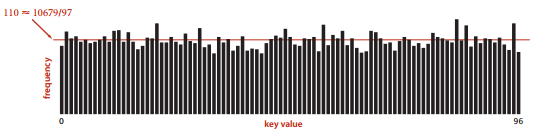
\includegraphics[scale=0.4]{{./figures/uniform_hashing}.png}

\smallskip

\tiny hash value frequencies for words in Tale of Two Cities (10,679 keys, $M = 97$)
\end{center}

\item collision: two distinct keys hash to the same index
\begin{itemize}
\item birthday problem $\implies$ can't avoid collisions unless you have
a ridiculous (quadratic) amount of memory

\item coupon collector + load balancing problems $\implies$ collisions are evenly distributed

\item challenge: deal with collisions efficiently
\end{itemize}
\end{itemize}
\end{frame}

\section{Separate-Chaining Symbol Table}
\begin{frame}[fragile]
\begin{itemize}
\item use an array of $M < N$ linked lists
\begin{itemize}
\item hash: map key to integer $i \in [0, M - 1]$

\item insert: put at front of $i$th chain (if not already there)

\item search: need to search only the $i$th chain
\end{itemize}

\begin{center}
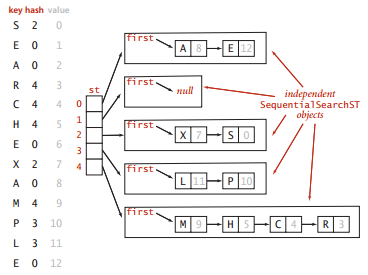
\includegraphics[scale=0.4]{{./figures/separate_chaining}.png}

\smallskip

\tiny hashing with separate chaining
\end{center}

\item the ratio $N / M$ is called the load factor and is denoted by $\alpha$; it is interpreted as the average number of keys per list
\end{itemize}
\end{frame}

\begin{frame}[fragile]
\begin{itemize}
\item under uniform hashing assumption, probability that the number of
keys in a list is within a constant factor of $\alpha$ is extremely close to 1

\item consequence: number of probes for search/insert is proportional to $\alpha$
\begin{itemize}
\item $M$ too large $\implies$ too many empty chains

\item $M$ too small $\implies$ chains too long
\end{itemize}

\item goal: $\alpha = $ constant
\begin{itemize}
\item double the size of array when $\alpha \geq 10$

\item halve the size of array when $\alpha \leq 2$

\item need to rehash all keys when resizing
\end{itemize}

\item deleting a key (and its associated value) is easy --- need only consider chain containing key
\end{itemize}
\end{frame}

\begin{frame}[fragile]
\begin{itemize}
\item implementation
\begin{lstlisting}[language=Java]
public class SeparateChainingHashST<Key, Value> implements ST<Key, Value> {
    private static final int INIT_CAPACITY = 4;
    private int N;
    private int M; 
    private LinkedST<Key, Value>[] st; 

    public SeparateChainingHashST() { this(INIT_CAPACITY); } 

    public SeparateChainingHashST(int M) {
        this.M = M;
        st = (LinkedST<Key, Value>[]) new LinkedST[M];
        for (int i = 0; i < M; i++) { st[i] = new LinkedST<Key, Value>(); }
    } 

    private void resize(int chains) {
        SeparateChainingHashST<Key, Value> temp = 
            new SeparateChainingHashST<Key, Value>(chains);
        for (int i = 0; i < M; i++) {
            for (Key key : st[i].keys()) {
                temp.put(key, st[i].get(key));
            }
        }
        this.M  = temp.M;
        this.N  = temp.N;
        this.st = temp.st;
    }
    
    public int size() { return N; } 

    public boolean isEmpty() { return size() == 0; }

    public boolean contains(Key key) { return get(key) != null; } 
    ...
}
\end{lstlisting}
\end{itemize}
\end{frame}

\begin{frame}[fragile]
\begin{itemize}
\item implementation (contd.)
\begin{lstlisting}[language=Java]
public class SeparateChainingHashST<Key, Value> implements ST<Key, Value> {
    ...
    public Value get(Key key) {
        int i = hash(key);
        return st[i].get(key);
    } 

    public void put(Key key, Value val) {
        if (val == null) {
            delete(key);
            return;
        }
        if (N >= 10 * M) { resize(2 * M); }
        int i = hash(key);
        if (!st[i].contains(key)) { N++; }
        st[i].put(key, val);
    } 

    public void delete(Key key) {
        int i = hash(key);
        if (st[i].contains(key)) { N--; }
        st[i].delete(key);
        if (M > INIT_CAPACITY && N <= 2 * M) { resize(M / 2); }
    } 

    public Iterable<Key> keys() {
        LinkedQueue<Key> queue = new LinkedQueue<Key>();
        for (int i = 0; i < M; i++) {
            for (Key key : st[i].keys()) { queue.enqueue(key); }
        return queue;
    } 
    ...
}
\end{lstlisting}
\end{itemize}
\end{frame}

\section{Linear-Probing Symbol Table}
\begin{frame}[fragile]
\begin{itemize}
\item use an array with $M > N$ slots
\begin{itemize}
\item hash: map key to integer $i \in [0, M-1]$

\item insert: put at array index $i$ if free; if not try $i+1$, $i+2$, etc

\item search: search array index $i$; if occupied but no match, try $i+1$, $i+2$, etc
\end{itemize}
\begin{center}
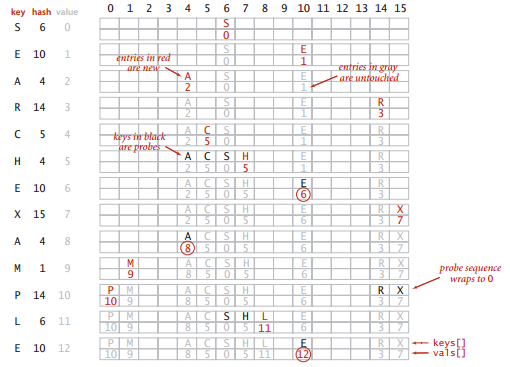
\includegraphics[scale=0.4]{{./figures/linear_probing}.png}

\smallskip

\tiny hashing with linear probing
\end{center}

\item the ratio $N / M$ is called the load factor and is denoted by $\alpha$; it is interpreted as the percentage of array slots that are occupied
\end{itemize}
\end{frame}

\begin{frame}[fragile]
\begin{itemize}
\item under uniform hashing assumption, the average number of probes
in a linear-probing symbol table that contains $N = \alpha M$ keys is $$\sim \frac{1}{2}\Big(1+\frac{1}{1-\alpha}\Big)$$
for a search hit, and $$\sim \frac{1}{2}\Big[1+\frac{1}{(1-\alpha)^2}\Big]$$ for a search miss/insert

\item consequence: when $\alpha$ is about $1/2$, the average number of probes for a search hit is about $3/2$ and for a search miss is about $5/2$
\begin{itemize}
\item $M$ too large $\implies$ too many empty array entries

\item $M$ too small $\implies$ search time blows up
\end{itemize}

\item goal: the load factor $\alpha < 1/2$.
\begin{itemize}
\item double size of array when $\alpha \geq 1/2$

\item halve size of array when $\alpha \leq 1/8$

\item need to rehash all keys when resizing
\end{itemize}

\item deleting a key (and its associated value) requires some care --- cannot just delete array entries
\end{itemize}
\end{frame}

\begin{frame}[fragile]
\begin{itemize}
\item implementation
\begin{lstlisting}[language=Java]
public class LinearProbingHashST<Key, Value> implements ST<Key, Value> {
    private static final int INIT_CAPACITY = 4;
    private int N; 
    private int M; 
    private Key[] keys; 
    private Value[] vals; 

    public LinearProbingHashST() { this(INIT_CAPACITY); }

    public LinearProbingHashST(int capacity) {
        M = capacity;
        keys = (Key[])   new Object[M];
        vals = (Value[]) new Object[M];
    }

    public int size() { return N; }

    public boolean isEmpty() { return size() == 0; }

    public boolean contains(Key key) { return get(key) != null; }

    private void resize(int capacity) {
        LinearProbingHashST<Key, Value> temp = 
            new LinearProbingHashST<Key, Value>(capacity);
        for (int i = 0; i < M; i++) {
            if (keys[i] != null) { temp.put(keys[i], vals[i]); }
        }
        keys = temp.keys;
        vals = temp.vals;
        M    = temp.M;
    }
    ...
}
\end{lstlisting}
\end{itemize}
\end{frame}

\begin{frame}[fragile]
\begin{itemize}
\item implementation (contd.)
\begin{lstlisting}[language=Java]
public class LinearProbingHashST<Key, Value> implements ST<Key, Value> {
    ...
    public void put(Key key, Value val) {
        if (val == null) {
            delete(key);
            return;
        }
        if (N >= M / 2) { resize(2 * M); }
        int i;
        for (i = hash(key); keys[i] != null; i = (i + 1) % M) {
            if (keys[i].equals(key)) { vals[i] = val; return; }
        }
        keys[i] = key;
        vals[i] = val;
        N++;
    }

    public Value get(Key key) {
        for (int i = hash(key); keys[i] != null; i = (i + 1) % M) {
            if (keys[i].equals(key)) { return vals[i]; }
        }
        return null;
    }
    ...
}
\end{lstlisting}
\end{itemize}
\end{frame}

\begin{frame}[fragile]
\begin{itemize}
\item implementation (contd.)
\begin{lstlisting}[language=Java]
public class LinearProbingHashST<Key, Value> implements ST<Key, Value> {
    ...
    public void delete(Key key) {
        if (!contains(key)) { return; }
        int i = hash(key);
        while (!key.equals(keys[i])) {
            i = (i + 1) % M;
        }
        keys[i] = null;
        vals[i] = null;
        i = (i + 1) % M;
        while (keys[i] != null) {
            Key   keyToRehash = keys[i];
            Value valToRehash = vals[i];
            keys[i] = null;
            vals[i] = null;
            N--;  
            put(keyToRehash, valToRehash);
            i = (i + 1) % M;
        }
        N--;        
        if (N > 0 && N <= M / 8) resize(M / 2);
    }

    public Iterable<Key> keys() {
        LinkedQueue<Key> queue = new LinkedQueue<Key>();
        for (int i = 0; i < M; i++) {
            if (keys[i] != null) { queue.enqueue(keys[i]); }
        }
        return queue;
    }
    ...
}
\end{lstlisting}
\end{itemize}
\end{frame}

\section{Performance Characteristics}
\begin{frame}[fragile]
\begin{itemize}
\item cost summary for symbol table implementations
\begin{center}
\begin{tabular}{ccc}
\textbf{operation} & \textbf{separate chaining} & \textbf{linear probing} \\ \hline \\
search & 3-5$^\dagger$ & 3-5$^\dagger$ \\
insert & 3-5$^\dagger$ & 3-5$^\dagger$ \\
delete & 3-5$^\dagger$ & 3-5$^\dagger$ \\
\end{tabular}  

\smallskip

\tiny $\dagger$ under uniform hashing assumption
\end{center}
\end{itemize}
\end{frame}

\end{document}
